\documentclass[border=4pt]{standalone}
\usepackage[T1]{fontenc}
\usepackage{helvet}
\renewcommand{\familydefault}{\sfdefault}
\usepackage{graphicx}
\usepackage{caption}
\usepackage{amsmath}
\captionsetup{font={sf,footnotesize},labelfont={sf,bf,footnotesize},justification=justified,singlelinecheck=false}
\begin{document}
\begin{minipage}{6.00in}
\centering
\begin{figure}[htbp]
    \centering
    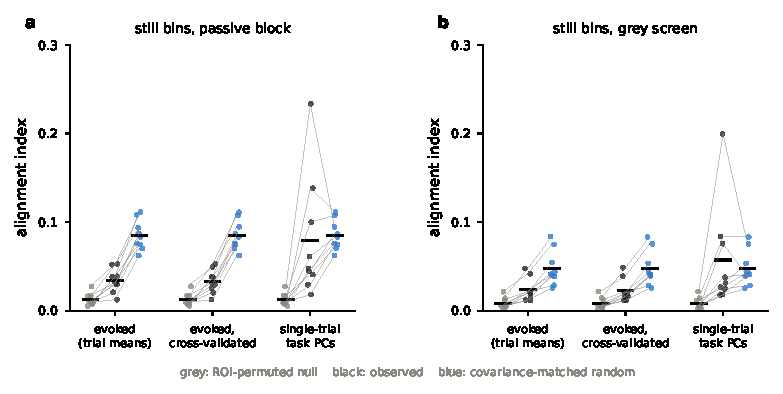
\includegraphics[width=\linewidth]{fig_repertoire_pilot_panels.pdf}
    \caption{Resting fluctuations in the mesoscope share the dims of task-period variability, but are not concentrated in the task-evoked patterns. \textbf{a} Alignment of resting fluctuations with task subspaces (K = 5 dims; uniform direction projected out), per mouse (dots; bars, means over 9 mice; lines connect a mouse). Rest: still 1\,s bins of the passive block (grey screen and receptive-field mapping), z-scored deconvolved activity of all ROIs, centred. Alignment index: rest variance in the subspace relative to the most any 5-dim subspace captures. Task subspaces: top dims of 16 trial-averaged evoked patterns (stim, choice, feedback, post-feedback windows minus pre-stimulus; side $\times$ outcome); the same restricted to dims shared by odd and even trials; top PCs of single-trial evoked activity (odd trials). Nulls: ROI permutation of the task patterns (grey) and random subspaces drawn from the covariance of all recording bins (blue). \textbf{b} The same for still bins of the grey screen alone (34 sessions).}
    \label{fig:repertoire_pilot}
\end{figure}
\end{minipage}
\end{document}
